\documentclass{beamer}
%\documentclass[aspectratio=169]{beamer}
%
\mode<presentation>
{
  \usetheme{default}      
  \usecolortheme{default}
  \usefonttheme{default} 
  \setbeamertemplate{navigation symbols}{}
  \setbeamertemplate{caption}[numbered]
} 

\usepackage[english]{babel}
\usepackage[utf8x]{inputenc}

\title[Course presentation]{Machine learning from scratch}
\subtitle{Lecture 1: Introduction and presentation of the course}
\author{Alexis Zubiolo\newline\texttt{alexis.zubiolo@gmail.com}}
\institute{Data Science Team Lead @ Adcash}
\date{\today}

\begin{document}

\begin{frame}
  \titlepage
\end{frame}

\begin{frame}{Before we start}
\vfill
I'd like to know a little bit more about you
\vfill
\begin{itemize}
	\item Short presentation: Name, occupation, \ldots
	\item Background in machine learning?
	\item Background in programming?
	\item Background in mathematics?
	\item Expectations from the course (if any)?
\end{itemize}
\vfill
Please send me an email so that I have your contact:
\vfill
\begin{center}
\texttt{alexis.zubiolo@gmail.com}
\end{center}
\vfill
All the material will be available on my personal GitHub:
\vfill
\begin{center}
\texttt{https://github.com/azubiolo/itstep}
\end{center}
\vfill
\end{frame}

\begin{frame}{Outline}
\vfill
\begin{itemize}
  \item What machine learning is, what it is not
\vfill
  \item A few practical examples
  \begin{itemize}
  	\item classification
  	\item regression
  \end{itemize}
\vfill
	\item Big picture of a machine learning algorithm
\vfill
  \item Goals and presentation of the course 
\vfill
  \item Questions and answers
\end{itemize}
\vfill

\end{frame}

\begin{frame}{What is machine learning?}
\vfill
A simple example\ldots
\vfill
\begin{figure}
\centering
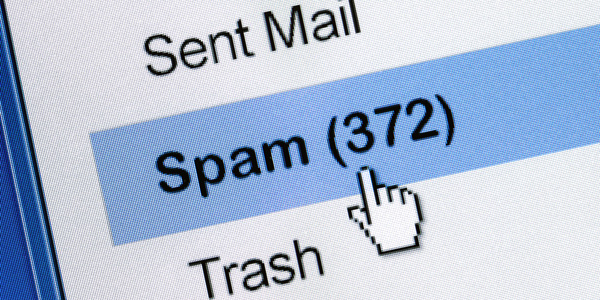
\includegraphics[width=\textwidth]{images/spam.jpg}
\end{figure}
\vfill
How to filter spam emails \textbf{automatically}?
\vfill
\end{frame}

\begin{frame}{Machine learning paradigm}
~\\
\vfill
Goal: Build algorithms that can 
\begin{itemize}
	\item \textbf{learn} from data
	\item \textbf{make predictions} on (new) data
\end{itemize}
\vfill
\pause
\begin{figure}
\centering
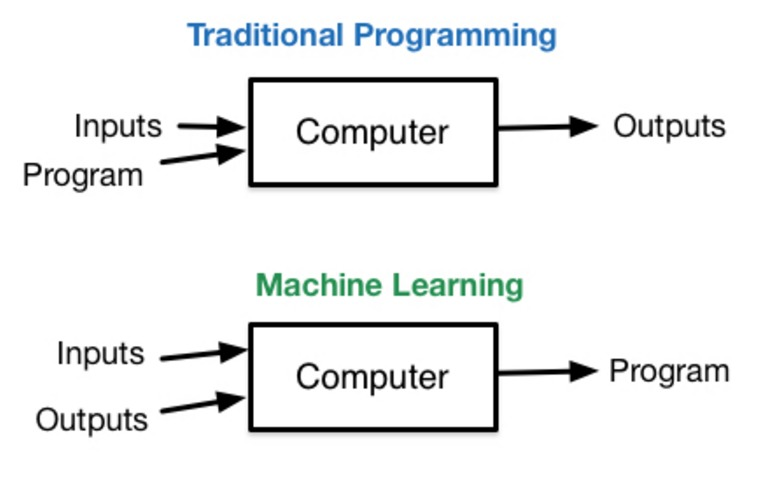
\includegraphics[width=\textwidth]{images/ml_vs_traditional.jpg}
\end{figure}
\vfill
\end{frame}

\begin{frame}{Main components of machine learning}
\vfill
\begin{itemize}
\item Mathematics
	\begin{itemize}
		\item Linear algebra
		\item Calculus
		\item Numerical optimization
	\end{itemize}
\vfill
\item Statistics, probability theory
\vfill
\item Computer science
\end{itemize}
\vfill
\pause
In the course, we will review these aspects.
\vfill
\textbf{Prerequisites}: I will assume
\begin{itemize}
	\item Some knowledge in computer science (understand: at least \textbf{a language you are comfortable with})
	\item You do not pass out when you see a mathematical formula
\end{itemize}
\vfill
\end{frame}

\begin{frame}{Example 1: Regression}

Regression = output is a \textbf{continuous} numerical value
\vfill
Example: \textbf{Estimate the price} of an apartment
\begin{itemize}
	\item input: \textbf{information} about the apartment
	\item output: \textbf{price}
\end{itemize}
\vfill
\pause
\begin{table}
\centering
\begin{tabular}{r|r}
living area (m$^2$) & price (1000's euros) \\\hline
50 & 30 \\
76 & 48 \\
26 & 12 \\
102 & 90 \\
\pause
61 & ?
\end{tabular}
\end{table}
\vfill
Linear model: price = \textbf{a} $\times$ area + \textbf{b}
\vfill
Problem: optimal values for \textbf{a} and \textbf{b}?

\end{frame}

\begin{frame}{Regression}

More data for a richer model:
\vfill
\begin{table}
\centering
\begin{tabular}{r|r|r}
living area (m$^2$) &  \textbf{\# bedrooms} & price (1000's euros) \\\hline
50 & \textbf{1} & 30\\
76 & \textbf{2} & 48\\
26 & \textbf{1} & 12\\
102 & \textbf{3} & 90\\
61 & \textbf{2} & ?
\end{tabular}
\end{table}

\vfill
\textbf{Linear model}: price = \textbf{a} $\times$ area + \textbf{b} $\times$ \# bedrooms + \textbf{c}
\vfill
\textbf{Problem}: Optimal values for \textbf{a}, \textbf{b} and \textbf{c}?
\vfill
\textbf{Remark}: More data does not always imply a better model
\end{frame}

\begin{frame}{Example 2: Classification}
\vfill
Classification = output is a \textbf{label}
\vfill
Examples: 
\pause
\vfill
\begin{itemize}
	\item Spam filtering
	\begin{itemize}
		\item input: email (text, subject, address, \ldots)
		\item output: \textbf{spam} or \textbf{not spam}
	\end{itemize}
\pause
\vfill
	\item Object recognition in images or videos
	\begin{itemize}
		\item input: image or video
		\item (example) output: \textbf{face} or \textbf{not a face}
	\end{itemize}
\pause
\vfill
	\item Image classification/description
	\begin{itemize}
		\item input: image
		\item output: image \textbf{description} or \textbf{label} (apple, car, \ldots)
	\end{itemize}
\end{itemize}
\vfill

\end{frame}

\begin{frame}{Automated image description generation}

\begin{figure}
\centering
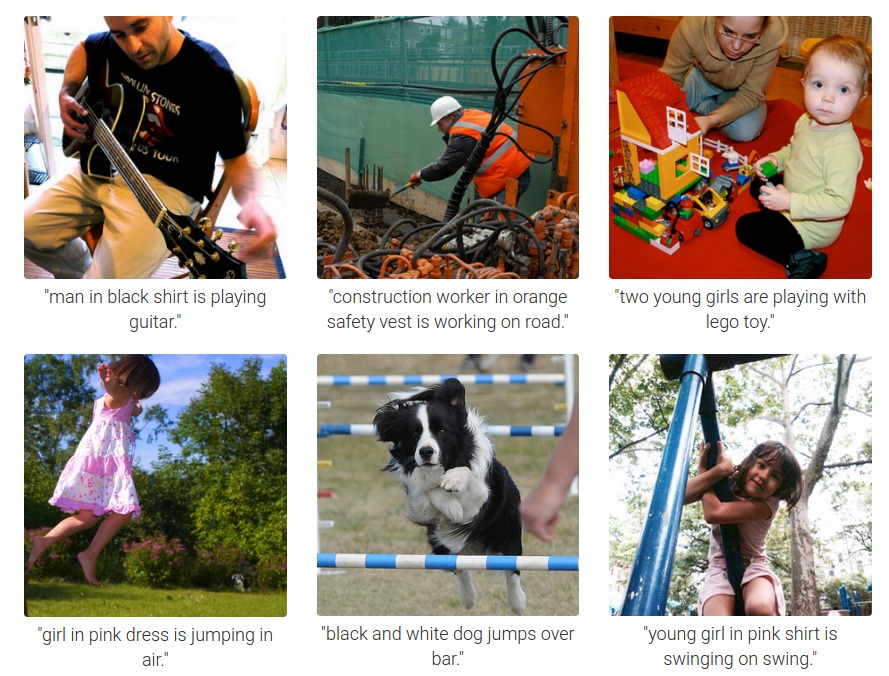
\includegraphics[width=\textwidth]{images/generated_descriptions.jpg}
\end{figure}
\end{frame}

\begin{frame}{Other topics}
\vfill
Machine learning is a wide and growing field. It also includes:	
\pause 
\vfill
\begin{itemize}
	\item Unsupervised learning/clustering (no predefined label/output)
\pause 
\vfill
	\item Dimensionality reduction
\pause 
\vfill
	\item Feature engineering
\pause 
\vfill
	\item \ldots
\end{itemize}
\vfill
This course will focus on \textbf{supervised learning}.
\vfill
\end{frame}

\begin{frame}{What machine learning is not}
Even though ML can provide great results, it is not a magic black box that solves all issues.
\vfill
ML users/engineers needs proper understanding and some experience 
\end{frame}

\begin{frame}{ML Algorithm: Big Picture}
There are several key steps when using supervised learning. Several pieces have to be wisely chosen:
\begin{itemize}
	\item A \textbf{data} set
	\item A \textbf{model}
	\item A \textbf{loss} function
	\item A \textbf{regularization}
	\item An \textbf{optimizer}
\end{itemize}
\vfill
\pause
These choices have to take into account a few constraints, depending on the application, \textit{e.g.}:
\begin{itemize}
	\item A minimum \textbf{accuracy} (or other performance index)
	\item \textbf{Time} constraints 
	\item \textbf{Resources} constraints (storage, computation power, architecture, \ldots)
\end{itemize}
\end{frame}

\begin{frame}{ML Algorithm}
In this course, we will focus on 
\begin{itemize}
	\item \textbf{Models}: linear, kernel, \ldots
	\item \textbf{Loss} functions: Least squares, logistic loss, \ldots
	\item \textbf{Regularization}: $\ell_2$ or $\ell_1$
	\item \textbf{Optimization} techniques: Stochastic/batch gradient descent
	\item \textbf{Evaluation} of models
\end{itemize}
\end{frame}

\begin{frame}{The course}
Goals:
\begin{itemize}
	\item Understand \textbf{how a supervised ML algorithm works}
	\item Being \textbf{able to implement a ML algorithm}
	\item Anything else you might have in mind
\end{itemize}
\vfill
\pause 
Practical information:
\begin{itemize}
	\item $\sim$ \textbf{10 60-90 min sessions} on Thursdays at 6:30 pm
	\item Starting with a few lectures about the main concepts followed by lab sessions where you implement these concepts
	\item All material will be \textbf{available on GitHub}, with links to extra material for those who want to go deeper
	\vfill
	\begin{center}
	\texttt{https://github.com/azubiolo/itstep}
	\end{center}
	\vfill
\end{itemize}
\end{frame}

\begin{frame}{Course outline (attempt)}
\vfill
\begin{itemize}
  \pause
  \item \textbf{Mathematical background}
  \begin{itemize}
  	\item Linear algebra (vector, matrices, operations)
  	\item Derivatives (gradient, Hessian matrix)
  	\item Convexity
  \end{itemize}
  \pause
  \item \textbf{Mathematical formalization of ML problems}
  \begin{itemize}
  	\item Linear models
  	\item Kernels
  	\item Loss functions (least squares, logistic regression, SVM)
  	\item Regularization
  \end{itemize}
  \pause
  \item \textbf{Optimization in machine learning}
  \begin{itemize}
  	\item Gradient descent
  	\item Stochastic vs. batch methods
  	\item Second-order methods
  	\item Learning rate
  \end{itemize}
  \pause
  \item \textbf{Model combination} (boosting)
  \pause
  \item \textbf{Model validation}
\end{itemize}
\vfill
\pause
\textbf{Note}: This is a first rough estimation. I will adapt to your needs and how fast things go.
\end{frame}

\begin{frame}{About programming languages}
For the practical sessions, I will be using \textbf{Python} with \textbf{Jupyter}.
\begin{center}
\texttt{http://jupyter.org/}
\end{center}
\vfill
If you prefer another language, feel free to use it. Remember that I assume some programming knowledge.
\end{frame}

\begin{frame}
\vfill
\centering
\begin{huge}
\huge{Thank you! Questions?}
\vfill
\texttt{alexis.zubiolo@gmail.com}
\end{huge}
\vfill
\begin{Large}
\texttt{https://github.com/azubiolo/itstep}
\end{Large}
\vfill
\end{frame}

\end{document}
